\chapter{Motivation}
\todo[inline]{Beispiel - Betz und Cacean\cite{ClimateEngineering, betz2012ethical}}
% Was sind Argumentkarten? Wer verwendet sie und wofür?
% Darstellung von Argumentkarten
% - Wie werden sie bis jetzt dargestellt?
% - Wieso will man sie darstellen?
Diese Arbeit beschäftigt sich mit Argumentkarten, manchmal auch Argumentationskarten genannt. Diese dienen als graphische Darstellung von Debatten. Eine Argumentkarte ist die Darstellung einer Debatte in Form eines Graphen.
Auf einer solchen Karte werden die Thesen und Argumente der Debatte als einzelstehende Elemente herausgestellt. 
Zusätzlich lassen sich auf solche einer Karte Beziehungen zwischen Argumenten, welche von unterstützenden oder angreifender Natur sein können, visualisieren.


%Debatten werden in der Regel in sogenannten Argumentkarten, manchmal auch Argumentationskarten, dargestellt. 
%Auf einer solchen Karte werden die Thesen und Schlüsse der Debatte in einzelne Sätze aufgeschlossen. Diese Sätze werden dann in einem Graphen abgebildet. 

% Spezielle Anforderungen
% - Wieso Gruppen?
% - Wieso Layout beibehalten? -> Mentale Karte
Die Argumentkarten sind vor allem ein Werkzeug zum besseren Verständnis der Debatte. 
Über die Visualisierung der Elemente und ihre Beziehungen hinaus, existieren weitere Möglichkeiten um das Verstehen der Debatte zu verbessern und zu erleichtern.
So können beispielsweise thematisch verwandte Knoten gruppiert werden. 
Auch durch die Option, Gruppen zunächst geschlossen zu visualisieren und Details zu verbergen, könnnen Gruppen einen schnelleren Überblick über die Debatte ermöglichen.
Das Hervorheben einzelner Argumentationsstrukturen durch die Wahl des Layouts ist eine weiterer wichtiger Aspekt bei der Visualisierung von Debatten.
%Dabei können verschiedene Aspekte der Debatte in den Vordergrund gerückt werden um diesen besser zu verstehen. 
%Beispielsweise können thematisch verwandte Knoten Gruppiert werden um einen besseren überblick über die Debatte zu ermöglichen 
%oder es können einzelne Arugmentationsstränge besonders hervorgehoben werden.

\begin{figure}[h]
\begin{center}
	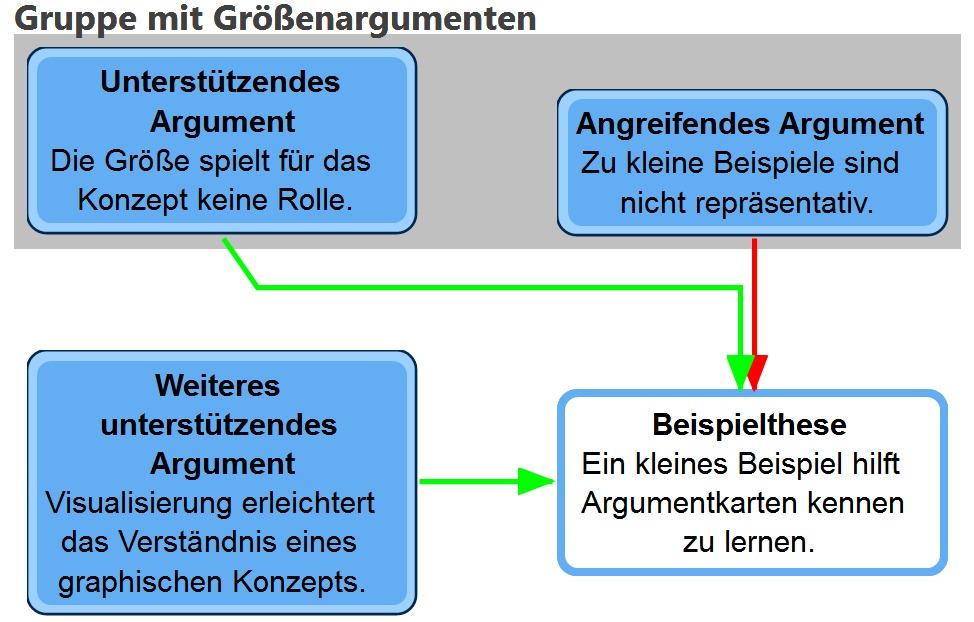
\includegraphics[width=0.5\textwidth]{Pics/Beispielargumentkarte.png}
	\caption{Beispielhafte Argumentkarte mit einer These, drei Argumenten und einer Gruppe.}
	\label{Beispielargumentkarte}
\end{center}
\end{figure}

Damit sich die von einer Argumentkarte bereitgestellten Informationen sinnvoll verwenden lassen, muss die Argumentkarte folglich auf eine geeignete Weise dargestellt werden.
Es existieren bereits einige Werkzeuge mit denen Argumentkarten angelegt  und ein Layout automatisch erzeugt werden kann. 
Allerdings müssen die resultierenden Layouts der Argumentkarten oftmals von Hand nachbearbeitet werden, um eine befriedigende Darstellung der Strukturen zu erhalten.
Darüber hinaus ist eine Unterstützung von Gruppen nicht immer gegeben.

% Wie ist diese Ausarbeitung aufgebaut?
%\subsection{Gliederung}
% 1. Problemstellung und -definition
% 2. Lösungsvorschlag
% 3. Detaillierte Erklärung des Algorithmus
% 4. Vergleich zu anderen Lösungsansätzen
In dieser Arbeit geht es um die automatisierte Darstellung von Argumentkarten mit Gruppen, sowie die Interaktion mit diesen Gruppen. 
%und damit um eine Möglichkeit die Argumentkarte zu vereinfachen um dem Benutzer einen schnellen und guten Überblick über die Debatte zu ermöglichen.
Es geht also um die Frage, wie sich Gruppen und Gruppenhierarchien den Anforderungen an Argumentkarten entsprechend visualisieren lassen 
und wie das Layout auf das Öffnen und Schließen von Gruppen reagiert.
%\todo[inline]{Lösungsanstz in Kurzform}

Im nächsten \autoref{chapter:layoutproblem}  präzisieren und abstrahieren wir diese Problemstellung. 
In \autoref{chapter:algo} präsentieren wir unseren Lösungsansatz, welchen wir dann in \autoref{chapter:vgl} mit alternativen Ansätzen vergleichen und bewerten.
\autoref{ch:zsf} schließt mit einer Zusammenfassung.



%-----------------------------------------------------------------------------------------------------------------------------------------------------------------------------------
\chapter{Problemstellung}%\chapter{Layoutproblem} % > mehr als Layout, betrachte auch Interaktion!
\label{chapter:layoutproblem}
\todo[inline]{Kapitelbeschreibung Korrekturlesen}
In diesem Kapitel beschäftigen wir uns im Allgemeinen wie eine Zeichnung einer Argumentkarte aussehen sollte.

\section{Layoutproblem}
\label{sec:layoutproblem}
% Was ist das grundlegende Problem? -> Layout finden
Das Zeichnen eines Graphen setzt sich aus dem Finden eines Layouts sowie des Renders zusammen. 
Für uns von Interesse ist nur ersteres, das Layoutproblem. 
Ziel hierbei ist es für einen gegebenen Graphen und gegebenenfalls weitere Informationen algorithmisch ein Layout zu berechnen,
welches gewisse Zeichenkonventionen erfüllt, erwünschte Ästhetikkriteren optimiert und gegebenenfalls weiteren lokalen Nebenbedingungen genügt.


% Was macht das Problem speziell? -> Gruppen und dass für Argumentkarten
% Was lässt sich jedoch abstrahieren? -> knoteninhalt, kanten
Im Fall der Argumentkarten abstrahieren wir für das Layoutproblem einige Informationen. 
So spielen die Texte der einzelnen These oder Argumente für uns keine Rolle. 
Sie werden lediglich durch achsenparallele Rechtecke als Knoten des Graphen repräsentiert.
Des Weiteren ignorieren wir bei den Beziehungen zwischen Elementen den Typ sowie die Richtung. 
Es ist also lediglich von Relevanz ob zwei Elemente in einer Beziehung stehen.
Dies wird dann durch eine ungerichtete Kante repräsentiert. 

Unter Einbeziehung von Gruppen kann die Eingabe des Algorithmus dann in der Form $G = (V,V_g,E,\sigma)$ dargestellt werden. Die Mengen und Abbildungen dieses Graphen werden im folgenden Beschrieben:
\todo[inline]{Baumstruktur}
\todo[inline]{Graph \& Abbildungen getrennt}
\begin{itemize}
	\item Knoten $V$, Knoten die eine Aussage repräsentieren.
	\item Gruppenknoten $V_g$, Knoten die eine Gruppe repräsentieren.
	\item Kanten $E \subseteq \bar{V} \times \bar{V}$, wobei $\bar{V}$ die Menge aller Knoten ($\bar{V} = V \cup V_g$) ist.
	%\item Rechtseindeutige Abbildung $\lambda(v): V \rightarrow B$, Die Knoten auf die Beschriftungsmenge $B$ (den Text der Knoten) abbildet.
	 \item Rechtseindeutige Abbildung $\sigma: \bar{V} \rightarrow V_g$, Die Knoten auf ihre Gruppe abbildet (Gruppen können weitere Gruppen enthalten).
\end{itemize}

%Zusätzlich zu dem so erhaltenen Graphen, haben wir Gruppen, 
%welche durch eine transitive, rechtseindeutige hierarchische Struktur von Gruppen von Knoten und Gruppen gegeben sind.
Bei Gruppen ist außerdem zu beachten, dass sie entweder in einem geöffneten oder geschlossen Zustand sein können.

%Wir erhalten also Eingabe zum einen Graphen  $G = (V, E)$ mit Knoten $V$, Kanten $E \subseteq V \times V$.
%, Knotenbeschriftungen $\lambda_{v}:V \rightarrow B_v$ und Kantenbeschriftungen $\lambda_{e}: E \rightarrow B_e$.

%Da es sich bei Argumentkarten um Graphen handelt ist die Darstellung einer Argumentkarte auch ein Layoutproblem.
%Anders als bei gewöhnlichen Graphen muss allerdings auch die Semantik des Graphen in die Zeichnung einfließen.
%%In unserem Fall beschränkt sich die semantische Betrachtung auf die Beziehungen von gruppierten Sätze und 
% > Falsche bzw nicht typischer Weg! Wenn dann nur nach Übersetzung von normalem Weg:
% Die Anforderungen an ein Layoutalgorithmus für die Darstellung von Argumentkarten mit Gruppen lassen sich demzufolge in allgemeine und in gruppensensitive Anforderungen Teilen.


%\section{Formale Beschreibung}
%\label{sec:formaldesc}
%Eine Argumentkarte lässt sich abbilden auf einen beschrifteten gerichteten Graphen.

%Ein solcher Graph $G = (V, E, \lambda_{v}, \lambda_{e})$ mit Knoten $V$, Kanten $E \subseteq V \times V$, Knotenbeschriftungen $\lambda_{v}:V \rightarrow B_v$ und Kantenbeschriftungen $\lambda_{e}: E \rightarrow B_e$. Dabei sind $B_v$ und $B_e$ die Beschriftungsmengen von Knoten bzw. Kanten.

%Auf einen solchen Graphen lässt sich lässt sich eine Argumentkarte Abbilden wenn die Kantenart als Kantenbeschriftung und der Knotentext als Knotenbeschriftung modelliert wird.

%Gegeben einem solchen beschrifteten gerichteten Graphen kann das Layouten eines Graphen als folgendes Problem modelliert werden:

%\begin{description}
%	\item[Eingabe] \hfill \\[0.3\baselineskip]
%			Beschrifteter gerichteter Graph $G = (V, E, \lambda_{v}, \lambda_{e})$ \hfill \\
			% = \{ \text{achsenparallele Rechtecke}\}
			%sowie einen Gruppenzugehörigkeitsbaum 
	
%	\item[Ausgabe] \hfill \\[0.3\baselineskip]
%		Zeichnung mit:
%		\begin{itemize}
%		\item $\forall x,y\in V, x \neq y: x \cap y = \emptyset$, also Knoten paarweise disjunkt
%		\item Überschneidungsfreiheit von Knoten: $\forall x, y \in V: x \neq y \Leftrightarrow x \cap y = \emptyset$
%		\item Überlagerungsfreiheit der Kanten: $\forall x, y \in E: x \neq y \Rightarrow \sigma(x, y) \leq 1$. Wobei $\sigma(x, y): E \times E \rightarrow \mathbb{N}_0$ eine Funktion ist, die für zwei Kanten $x$ und $y$ die Anzahl der Schnittpunkte angibt.
				%$\forall x \in V, (y,z) \in E, y\neq x\neq z: x \cap (y,z) = \emptyset$, also Kanten schneiden nur inzidente Knoten
%		\item Sonstige Nebenbedingung (Layoutanforderungen)
%	\end{itemize}
%\end{description}

% > Semantik spielt im ganzen Layout keine Rolle! Gruppen sind keine Semantik
\paragraph{Zeichenkonventionen}
Zeichenkonventionen beschreiben wie Knoten und Kanten gezeichnet beziehungsweise gelayoutet werden sollen. Sie müssen erfüllt werden.
In unserem Fall sind diese Anforderungen im einzelnen:

\begin{itemize}
\item Knoten $V$ werden als achsenparallel Rechtecke dargestellt
\item Überschneidungsfreiheit von Knoten
\item Überschneidungsfreiheit von Kanten mit Knoten
\item Eine geschlossene Gruppe enthält keine Knoten
\end{itemize}

Für unseren Lösungsansatz haben wir für Gruppen weitere Zeichenkonvention hinzugefügt:
\begin{itemize}
\item Gruppen werden als Kreise dargestellt
\item Eine geöffnete Gruppe beinhaltet alle Kindknoten sowie Kindgruppen
\item Überschneidungsfreiheit von Gruppen mit nicht Kindknoten oder -gruppen, sowie Kanten zwischen solchen
\end{itemize}

\paragraph{Ästhetikriterien}
Ästhetikkriterien sollen vom berechneten Layout optimiert werden. 
Auch wenn es für Argumentkarten im Allgemeinen wünschenswert ist, haben wir in unserem Lösungsansatz die Kreuzungsminimierung nicht beachtet.
\begin{itemize}
\item Größenminimierung 
\item Kreuzungsminimierung
\end{itemize}

Lokale Nebenbedingungen haben wir für das Layoutproblem nicht definiert.


%\section{Layoutanforderungen}
%Da es sich bei Argumentkarten um Graphen handelt ist die Darstellung einer Argumentkarte auch ein Layoutproblem.
%Anders als bei gewöhnlichen Graphen muss allerdings auch die Semantik des Graphen in die Zeichnung einfließen.
%In unserem Fall beschränkt sich die semantische Betrachtung auf die Beziehungen von gruppierten Sätze und 
%Zusätzlich zu den in \autoref{sec:formaldesc} beschriebenen Anforderungen muss die Zeichnung noch weitere ästhetische und funktionale Layoutanforderungen erfüllen die wir im %folgenden in allgemeine und Gruppensensitive Layoutanforderungen aufteilen.
% > was genau willst du damit für das Layout definieren?
%\subsubsection{Verständlichkeit} 
%Derzeitig werden sowohl die Gruppen in Argumentkarten von Hand erstellt als auch deren Darstellung im Layout der Argumentkarte. Die Gruppierung dient dabei maßgeblich dem %Verständnis der Argumentkarte und beruht und hilft es die Argumentkarte leichter zu verstehen unter dem Aspekt der Begrenztheit des menschlichen Kurzzeitgedächtnisses. % > das stimmt ja wohl nicht. scheiß auf begrenztheit des kurzzeitgedächtnis in diesem fall... :D
%(siehe \cite{miller1956magical, BBS:84441}).

%Ein entsprechender Layoutalgorithmus muss in der Lage sein die Gruppen so darzustellen, das die Beziehung der Gruppe zum Rest der Argumentkarte verständlich bleibt.
\todo[inline]{Beschreibung wie Zeichnung aussehen soll}
\section{Interaktion mit Gruppen}
\todo[inline]{Referenz Layout adjustment and the mental map}
% was ist außerdem ein Problem? -> Interkation
Da Gruppen sowohl geöffnet als auch geschlossen sein können, existieren eine Vielzahl von verschiedenen Layouts für eine Argumenkarte.
Außerdem sollte in einer Implementierung das Wechseln zwischen den verschiedenen Zuständen möglich sein, also das Öffnen und Schließen von Gruppen. 
Dadurch soll es zum einen einfach sein sich einen Überblick zu verschaffen und zum anderen eine detailliertere Ansicht zu haben.
% welche Anforderungen haben wir daran? -> nachvollziehbarkeit / beibehalten der mentalen Karte
Hierbei ist höchst wünschenswert, dass bei einer solchen Interaktion das alte und neue Layout nur so wenig wie möglich und nur so viel wie nötig unterscheiden. 
Der Nutzer soll sich mit seiner mentalen Karte der Argumentkarte auch nach der Interaktion zurechtfinden können.

Eine weitere wünschenswerte Anforderung ist, dass das Layout nach wiederholten Auf- und Zuklappzyklen immer wieder zu dem gleichen Anfangslayout oder dazu ähnlichem Layout zurückkehrt.

Wir erhalten für eine Interaktion und das Verhältnis der einzelnen berechneten Layouts also weitere Kriterien:
\begin{itemize}
\item Relative Positionen von Elementen verändert sich nur so viel wie nötig
\item Gesamtlayout ändert sich nur so viel wie nötig
\item Layout eines Zustandes ist auch nach mehreren Interaktionen das gleiche oder sehr ähnlich
\end{itemize}
% Verhalten beim Öffnen oder Schließen von Gruppen
% - Vorgaben an Verhalten: 
	% Ästhetikkritieren
	% - relative Positionen von Knoten und Gruppen verändern sich nur wenig
	% - Stuktur vor Zustandsänderung bleibt ähnlich und wiedererkennbar

Hierbei sei auch angemerkt, dass im Folgenden die Beziehungen der einzelnen Layouts, also die einzelnen Layouts von verschiednen Konfigurationen von auf- bzw. zugeklappten Gruppen, so aufgefasst werden, dass wir ein einziges Layout haben und dieses durch eine Interaktion in einen anderen Zustand wechselt.


Aus diesen und den in \autoref{sec:layoutproblem} vorgestellten Anforderungen ergibt sich allerdings eine Reihe von Konflikten.
Beispielsweise steht die Größenminimierung der Zeichnung im Konflikt mit der Anforderung, dass sich das Gesamtlayout nur so viel wie nötig ändert, 
da größenminimale Layouts nach dem Öffnen bzw. Schließen einer Gruppe möglicherweise nur mit einer großen Veränderung des Layouts möglich sind.

Der im Folgenden präsentierte Ansatz gibt schlägt jedoch Problemlösungen vor oder präferiert eine der Optionen.

\todo[inline]{Diskussion Consistent Label - Been et al}
%Ein weiteres Beispiel sind die Anforderungen an Überschneidungsfreiheit von Knoten mit Kanten und die Kreuzungsminimierung, da eine Möglichkeit die Anzahl der Kreuzungen zu reduzieren die Überlagerung von Knoten mit Kanten wäre.

%Der im Folgenden vorgestellten Lösungsansatz sowie die Alternativen in \autoref{chapter:vgl}


%\todo[inline]{Zusammenhang der Probleme hervorheben. Interkation hat Einfluss auf Wahl des Layouts, etc.}
% --------- 
%\subsubsection{Nachvollziehbarkeit}
%Zusätzlich zur Verständlichkeit muss das Layout auch Nachvollziehbar sein. % > was soll das heißen? wann ist den ein layout nachvollziehbar? O_o
%Zur Nachvollziehbarkeit gehört sowohl die Nachvollziehbarkeit einer statischen Abbildung der Argumentkarte, 
% richtig: ... wie auch die Nachvollziehbarkeit von Änderungen an dieser Abbildung.

%Damit eine statische Abbildung nachvollziehbar ist muss diese die von der Gruppe verschleierten Informationen, % > verschleiert :D
%wie Größe oder Relation der Gruppenmitglieder zum Rest der Argumentkarte durch geeignete Darstellung der Gruppe angedeutet werden.



% > das ist falsch. änderungen können nicht kleiner vorgenommen werden, als notwendig! 
% > richtig:  eine änderung hat nur geringen einfluss auf das gesamte layout hat und mentale karte bleibt erhalten
%Nachvollziehbar ist eine daraus resultierende Änderung des Graphen dann, wenn sie in kleinen Schritten erfolgt. 
%Dies bedeutet in unserem Fall, dass das Auf- und Zuklappen von Gruppen den Graphen die Gesamtstruktur der Zeichnung nur in relativ kleinen Schritten verändern soll.

%nun oben | Zur Nachvollziehbarkeit gehört aber auch das das Layout nach wiederholten Auf- und Zuklappzyklen immer wieder zu einem dem Anfangslayout ähnlichen Layout zurückkehrt.


%\todo[inline]{Problem definieren, Layoutproblem und Subprobleme, Layoutanspassungsproblem} Wir können für diese Problem ein Layoutproblem definieren.

%\begin{description}
%\item[Eingabe] Gegeben ein Graph $G=(V,E)$ mit Knoten $V = \{ \text{achsenparallele Rechtecke}\}$ und  Kanten $E \subseteq V \times V$,
%sowie einen Gruppenzugehörigkeitsbaum 
%
%\item[Zeichenkonvetionen]
%	\begin{itemize}
%	\item Geradlinige Kanten
%	\item $\forall x,y\in V, x \neq y: x \cap y = \emptyset$, also Knoten paarweise disjunkt
%	\item $\forall x \in V, (y,z) \in E, y\neq x\neq z: x \cap (y,z) = \emptyset$, also Kanten schneiden nur inzidente Knoten
%	\end{itemize}
%
%\item[Ästhetikkriterien]
%
%\item[Lokale Nebenbedingungen]
%
%\end{description}
%
%\section{Lösungsansätze}

% Layoutproblem
% - Gegeben/Eingabe und Abstraktion
	% Graph mit Knoten $V = \{ \text{achsenparallele Rechtecke}\}$, und  Kanten $E \subseteq V \times V$
	% sowie transitive, rechtseindeutige hierarchische Struktur von Gruppen von Knoten und Gruppen
	% Zustand, welche Gruppen offen/zu
	% Anfangslayout (!?)
% - Vorgaben an Layout: 
	% Zeichenkonventionen, hard constraints:
	% - Knoten und Knoten überschneiden sich nicht (jedoch dürfen Kanten Gruppen schneiden, wenn sie zu Element der Gruppe gehören)
	% - Gruppen umschließen alle ihre Elemente (welche zusammengeklappt halt in einem Punkt zusammenfallen)
	% Ästhetikkritieren
	% - Kreuzungsminimierung
	% - gleichmäßige Kantenlängen (?)
	% - Wendepunktminimierung von Kanten
	% - Struktur hervorheben in Gruppen (?)
	% Lokale Nebenbedingungen
	% - Nummerierung von Nachbarknoten im Layout repräsentieren
	


	
% Gewählter Zeichenstil
% - Argumente als Rechtecke (mit fester Breite?)
% - Gruppen als Kreise
% - Kanten als ``glatte'' Kurven (bis zu welchem Grad?)
% - Kanten in Gruppen rein/aus Gruppe raus zu/von inneren Elementen nur über Ports
